\section{The Friedmann equations}
We now want to determine the dynamics of the parameters appearing in the Friedmann Robertson Walker \eqref{eq:RWMetric} metric knowing the energy content of the universe. The connection between the metric and the energy is given by the \emph{Einstein field equations}
\begin{equation}\label{eq:EFE}
    R_{\mu\nu}-\frac{1}{2}Rg_{\mu\nu}=8\pi GT_{\mu\nu},
\end{equation}
where it appears the energy-momentum tensor $T^{\mu\nu}$. To solve this equation a specific energy momentum tensor must be chosen, thus a specific model of the universe content.
\subsection{Cosmic fluids}
The simplest model for the content of the universe is a \emph{perfect fluid} of energy and matter. A perfect fluid, in general, is described by an energy-momentum tensor given by
\begin{equation}\label{eq:PerfectFluidEMTensor}
    T^{\mu\nu}=(\rho+p)U^\mu U^\nu+pg^{\mu\nu},
\end{equation}
where $\rho$ is the energy density of the fluid, $p$ the pressure and $U^\mu$ the $4$-velocity of associated to the bulk motion of the fluid.\\When we described the coordinates appearing in the FRW metric, we anticipated that those were comoving coordinates with respect to the content of the universe (so that in that reference frame the metric would be manifestly isotropic and homogeneous). In the reference frame associated to those coordinates, the fluid is at rest\footnote{Note that the fluid must be at rest to satisfy the cosmological principle, its single particles can move randomly without spoiling isotropy and homogeneity microscopically.}, thus its energy-momentum tensor takes the form
\begin{equation}
    U^\mu=(1,0,0,0),\quad\Rightarrow\quad
    T_{\mu\nu}=\begin{pmatrix}
        \rho&0&0&0\\
        0&&&\\
        0&&g_{ij}p&\\
        0&&&
    \end{pmatrix},
    \quad T^\mu\phantom{} _\nu=\text{diag}(-\rho,p,p,p)\label{eq:EMTensorCosmicFluid}
\end{equation}
Even before plugging everything in the Einstein equations, we can study the energy conservation of this fluid, which reads
\begin{align}\label{eq:ConservationEnergy}
    0&=\nabla_\mu T^\mu\phantom{} _0=\partial_\mu T^\mu\phantom{} _0+\Gamma^\mu_{\mu\lambda}T^\lambda\phantom{} _0-\Gamma^\lambda_{\mu0}T^\mu\phantom{} _\lambda=\partial_0 T^0\phantom{} _0+\Gamma^\mu_{\mu0}T^0\phantom{} _0-\Gamma^\lambda_{\mu0}T^\mu\phantom{} _\lambda\nonumber\\
    &=-\dot\rho-3\frac{\dot a}{a}\rho-3\frac{\dot a}{a}p=-\dot\rho-3\frac{\dot a}{a}(\rho+p),
\end{align}
where we used that $T^\mu\phantom{}_\nu$ is diagonal, and the Christoffel symbols \eqref{eq:RWChristoffel}.\\
For simple fluids, it is usually assumed that they follow some simple equation of state, as
\begin{equation}\label{eq:EquationState}
    p=\omega\rho,\qquad\omega=\text{constant}.
\end{equation}
Inserting this into the conservation of energy equation \eqref{eq:ConservationEnergy} we find
\begin{equation*}
    \frac{\dot\rho}{\rho}=-3(1+\omega)\frac{\dot a }{a},
\end{equation*}
that can be solved to obtain how the energy density of the fluid scales as the universe expands:
\begin{align*}
    \int \frac{d\rho}{\rho}=-3(1+\omega)\int \frac{da}{a} \quad\Rightarrow\quad \boxed{\rho=\rho_0a^{-3(1+\omega)}}.
\end{align*}
To better grasp the physics of our construction let's study some simple cases.
\begin{itemize}
    \item \textbf{Dust}: this kind of fluid is defined as a set of collisionless, non-relativistic particles, that therefore will have zero pressure:$$p_d=\omega_d\rho_d=0,\quad\Rightarrow\quad \omega_d=0\quad\Rightarrow\quad\rho_d=\frac{E}{V}=\rho_{0}a^{-3}.$$ We can appreciate how, for dust, the energy density scales with the volume ($V \propto  a^3$), keeping constant the total energy. This fluid can be used to model cold matter, for which the pressure is negligible, such as cold dark matter or baryons after cosmological recombination (see Section \ref{sec:LambdaCDM}).
    \item \textbf{Radiation}: in this case we want to describe massless particles or ultra-relativistic ones, which can be approximated to be massless. We can obtain an equation of state for this fluid by first observing that the $T^{\mu\nu}$ is traceless for E-M fields $$T^\mu\phantom{}_\mu=F^{\mu\lambda}F_{\mu\lambda}-\frac{1}{4}g^\mu\phantom{}_\mu F^{\lambda\sigma}F_{\lambda\sigma}=0,$$ at the same time equation \eqref{eq:EMTensorCosmicFluid} gives that $$T^\mu\phantom{}_\mu=-\rho+3P,\quad\Rightarrow\quad P_r=\frac{1}{3}\rho_r,$$ which implies $\omega_r=\frac{1}{3}$. Therefore, the energy density of radiation scales as$$\rho_r=\rho_0a^{-4},$$ that means that for radiation the total energy is not constant in time. We interpret this as the fact that, while the universe expands, radiation gets redshifted.
    \item \textbf{Vacuum or dark energy}: this last type of cosmic fluid is quite a strange one, the equation of state for this fluid is $$p_v=-\rho_v,\quad \Rightarrow\quad \omega_v=-1.$$ This means that the energy density, as well as the pressure, as the universe expands, remains constant. The \emph{cosmological constant} $\Lambda$ can be interpreted as such a fluid, for which its energy density turns out to be: $$\rho_v=\frac{\Lambda}{8\pi G}.$$
\end{itemize}
\subsection{The Friedmann equations}
Now that we know how to model the content of the universe, we can proceed to derive the equations governing the time evolution of spacetime. First we want to modify a bit Einstein equations \eqref{eq:EFE}: from the trace of both sides we get
\begin{equation*}
    R-\frac{4}{2}R=8\pi GT\quad\Rightarrow\quad R=-8\pi GT,
\end{equation*}
where $T=T^\mu\phantom{}_\mu$, plugging this result in the field equations \eqref{eq:EFE}, we can rewrite them as:\begin{equation*}
    R_{\mu\nu}=8\pi G\bigg(T_{\mu\nu}-\frac{1}{2}Tg_{\mu\nu}\bigg).
\end{equation*}
From the Ricci tensor components of the FRW metric \eqref{eq:RWRicci} and the energy momentum tensor \eqref{eq:EMTensorCosmicFluid} we can obtain two equations:
\begin{itemize}
    \item the $\mu\nu=00$ component leads to
    \begin{align*}
        -3\frac{\ddot a}{a}&=8\pi G\bigg[-\rho-\frac{1}{2}(-\rho+3p)\bigg]\\&=4\pi G(\rho+3p);
    \end{align*}
    \item the $\mu\nu=ij$ components lead to
    \begin{align*}
        \frac{a\ddot a+2\dot a^2+2k}{a^2}g_{ij}&=8\pi G\bigg[pg_{ij}-\frac{1}{2}g_{ij}(-\rho+3p)\bigg]\\&=4\pi G(\rho-p)g_{ij}.
    \end{align*}
\end{itemize}
Substituting the former into the latter we find
\begin{align}
   -\frac{4}{3}\pi G(\rho+3p) +\frac{2\dot a^2+2k}{a^2}&=4\pi G(\rho-p)\nonumber\\\frac{2\dot a^2+2k}{a^2}&=4\pi G\frac{4}{3}\rho\quad\Rightarrow\quad  \boxed{\bigg(\frac{\dot a }{a}\bigg)^2=\frac{8\pi G}{3}\rho-\frac{k}{a^2}}\label{eq:Friedmann1},
\end{align}
which is the \textbf{first Friedmann equation}. From the $00$ component alone we get the \textbf{second Friedmann equation}
\begin{equation}
    \label{eq:Friedmann2}\boxed{\frac{\ddot a}{a}=-\frac{4\pi G}{3}(\rho+3p)}.
\end{equation}
The first, which is the one that is usually referred as the Friedmann equation, will determine the time evolution of the scale factor $a(t)$. Note that again we have more equation of motion than the number of degrees of freedom that we have to solve for: this is something that we must expect from a constrained system as general relativity. Indeed, equation \eqref{eq:Friedmann1} is just a constraint on the scale factor. However, it is well known from the theory of constrained Hamiltonian systems, that the constraint itself can be used to determine the dynamics of the system without employing the equation of motion. Using the first Friedman equation has the advantage of being a first order differential equation and that only the energy density has to be used. As we are going to see, solutions to this equation will depend on the explicit for of the energy density $\rho$ as a function of the scale factor, which we already determined in the case of single-component fluids in the previous section.  

Usually, the first Friedmann equation \eqref{eq:Friedmann1} is expressed in terms of specific cosmological parameters that are closer to observations:
\begin{itemize}
    \item the \textbf{Hubble parameter}, $H\defeq\frac{\dot a}{a}$, which measure the rate of expansion,
    \item the \textbf{critical density}, $\rho_{\text{crit}}\defeq\frac{3H^2}{8\pi G},$ which is the energy denisty of a flat universe,
    \item the \textbf{density parameter}, $\Omega=\frac{8\pi G}{3H^2}\rho\defeq\frac{\rho}{\rho_{\text{crit}}}$, 
    \item the \textbf{curvature parameter}, $\Omega_k\defeq\frac{k}{(aH)^2}$.
\end{itemize}
In this way, equation \eqref{eq:Friedmann1} explicitly relates the matter content of the universe with its geometry (flat. open or closed). Indeed, inserting the above parameters in \eqref{eq:Friedmann1} it reads
\begin{equation}\label{eq:Friedmann_Omega}
    \boxed{\Omega-1=\Omega_k=\frac{k}{H^2a^2}},
\end{equation}
from which we can distinguish 3 distinct cases:
\begin{itemize}
    \item $\rho<\rho_{\text{crit}}\quad\Leftrightarrow\quad \Omega<1 \quad\Leftrightarrow\quad k<0 \quad\Leftrightarrow\quad $\emph{open universe},
    \item  $\rho=\rho_{\text{crit}}\quad\Leftrightarrow\quad \Omega=1 \quad\Leftrightarrow\quad k=0 \quad\Leftrightarrow\quad $\emph{flat universe},
    \item  $\rho>\rho_{\text{crit}}\quad\Leftrightarrow\quad \Omega>1 \quad\Leftrightarrow\quad k>0 \quad\Leftrightarrow\quad $\emph{closed universe}.
\end{itemize} 
As we will see, observations suggest that now, for our universe, $\Omega_k\approx0$. Therefore, we will always consider flat geometry, in this case the dynamics of the universe is determined by $$\bigg(\frac{\dot a }{a}\bigg)^2=\frac{8\pi G}{3}\rho. $$
In general all fluids will make up the total energy density of the universe, however solving for the exact dynamics in this case becomes almost impossible. We therefore resort to the approximation of a universe filled by a single fluid, which in reality is the dominant one (its energy density) at a given time. In this way we recognize three main cases. 
\begin{itemize}
    \item \textbf{Matter dominated universe}: in this case, the universe is approximated to contain only dust, therefore $\rho=\rho_0a^{-3}$. Plugging this energy density into the above differential equation we get$$\dot a=H_0a^{-\frac{1}{2}}\quad \Rightarrow\quad a(t)=\bigg(\frac{3}{2}H_0t\bigg)^{2/3},$$ where $H_0=H(t_0)=\sqrt{\frac{8\pi G}{3}\rho_0}$ and we imposed $a(0)=0$.\\ This kind of universe is expanding but at a slower and slower rate ($\ddot a\leq0$).
    \item  \textbf{Radiation dominated universe}: assuming that the universe is approximately filled only by radiation, therefore $\rho=\rho_0a^{-4}$, the above differential equation now reads$$\dot a=H_0a^{-1}\quad \Rightarrow\quad a(t)=\sqrt{2H_0t},$$ where again $H_0=H(t_0)=\sqrt{\frac{8\pi G}{3}}$ and $a(0)=0$.\\ Again, this universe is expanding at a slower and slower rate ($\ddot a\leq0$).
    \item \textbf{Empty universe}: lastly we consider an empty universe or in which vacuum energy dominates, therefore $\rho=\frac{\Lambda}{8\pi G}$, from which we get$$\dot a=a\sqrt{\frac{\Lambda}{3}}\quad \Rightarrow\quad a(t)=a_0e^{\sqrt{\frac{\Lambda}{3}}(t-t_0)},$$
     in which this time we imposed $a(t_0)=a_0$.\\Note that, among the cases, this universe is the only one that has an accelerating expansion ($\ddot a\geq0$). It is worth noting also that the first two cases admit a finite time (in our calculations $t=0$) for which the universe has no spatial extension ($a(0)=0$). The empty universe does not admit it for any finite time. 
\end{itemize}
\begin{figure}
    \centering
    \label{fig:a_comparison}
    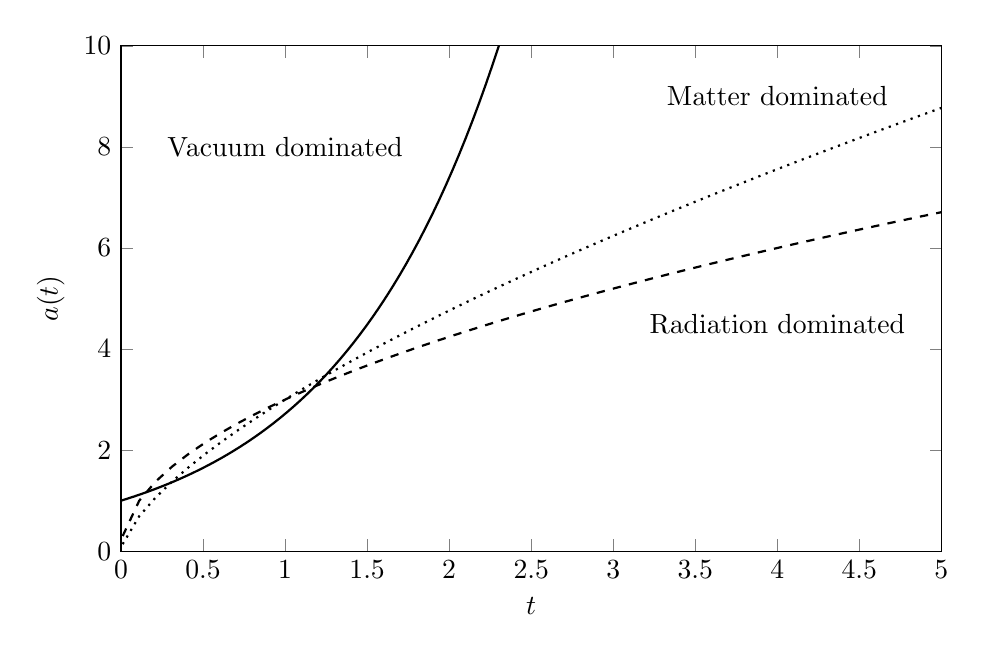
\begin{tikzpicture}[scale=1]
        \begin{axis}[
            width=12cm, height=8cm,
            xlabel={$t$}, ylabel={$a(t)$},
            xmin=0, xmax=5,
            ymin=0, ymax=10,
            legend pos=north east,
            legend style={font=\small}
        ]
            % Plot for a_mat = t^(2/3)
            \addplot[
                domain=0.01:10, % Avoid t=0 for power functions
                samples=100,
                thick,
                dotted
            ] {3*x^(2/3)};

            % Plot for a_rad = t^(1.5)
            \addplot[
                domain=0.01:10,
                samples=100,
                thick,
                dashed
            ] {3*x^(0.5)};
            

            % Plot for a_vac = e^t
            \addplot[
                domain=0:4,
                samples=100,
                thick,
            ] {exp(x)};
            \node at (axis cs:4,4.5) {Radiation dominated};
            \node at (axis cs:4,9) {Matter dominated};
            \node at (axis cs:1,8) {Vacuum dominated};
        \end{axis}
    \end{tikzpicture}
    \caption{Comparison of the time evolution of the scale factor with the three different fluids in a flat universe. Only the vacuum dominated universe (solid line) displays an accelerating expansion. Arbitrary units are used in this plot.}
\end{figure}
\subsection{The $\Lambda$CDM model} 
\label{sec:LambdaCDM}
With all the previous tools we introduced we are finally ready to describe the universe that we live in and its evolution. To draw the timeline of our universe we must start from today, from current observations of the cosmological parameters, and then trace back its history.

The first cosmological parameter that has been ever observed is the Hubble parameter, by Hubble himself. Current and more precise measurements \cite{planck2018results} of this parameter give
$$H_0=(67.36\pm0.54)\text{km s$^{-1}$Mpc$^{-1}$}$$
which correspond to a critical density of roughtly $\rho_{\text{crit},0}=8.6\times10^{-27}\text{kg m}^{-3}$.

Nowadays, most of our knowledge on cosmology comes from measurements of the \emph{CMB}, or the \emph{Cosmic Microwave Background radiation}, which (for now) is (just) the relic of the photons that filled the universe at earlier times. In $1996$, the \emph{COBE} satellite \cite{COBE1996} measured the spectrum of the CMB as an almost perfect blackbody radiation at the temperature 
\begin{equation}
    \label{eq:T0_CMB}
    T_0=(2.7255\pm0.0006)K,
\end{equation}
this allows to estimate the number density and the energy density of these relic photons (Section \ref{sec:EquilibriumDistributions}) that read
\begin{equation}
    n_{\gamma,0}\approx410\text{ photons cm}^{-3},\quad \rho_{\gamma, 0}\approx4.6\times10^{34}\text{g cm}^{-3},\quad\Omega_{\gamma,0}=(5.38\pm0.15)\times10^{-5}.
\end{equation}
This turns out to be the main contribution to all the photon contained in the universe.\\
By the results of COBE, we also discovered that the CMB displays small temperature anisotropies $\Delta T/T\approx 10^{-5}$ that, we will see, give us a tremendous amount of data about the history of the universe. For now, it is important that these measures suggest an upper bound for the spatial curvature of our universe today (as measured by the Planck collaboration \cite{planck2018results})
\begin{equation}
    \label{eq:Omega_k0}|\Omega_{k,0}|<0.005.
\end{equation}
This shows that today only a small fraction of all the contribution to the Friedmann equation \eqref{eq:Friedmann_Omega} is represented by curvature and therefore we consider our universe almost flat. 

Together with photons, our universe is also filled with neutrinos that, being really light particles, behave almost as radiation (their speed is really close to $c$)\footnote{In this context radiation means that we describe this fraction of energy as a perfect fluid with $\omega=1/3$.}. The total contribution of the three massless neutrinos predicted by the \emoh{Standard Model} and photons energy density is (as one can derive by Plank results \cite{planck2018results})  
\begin{equation}
    \Omega_{r,0}=(9.29\pm0.21)\times10^{-5}.
\end{equation}

Clearly, also the ordinary matter of which we are made of (what we called dust that mainly is stars and gasses that fill the universe) must be taken into account: current measures \cite{planck2018results} from the CMB, by the Planck collaboration, and the abundances of the lightest chemical elements in our universe show 
\begin{equation}
    \Omega_{b,0}=0.0493\pm0.0003,
\end{equation}
where the subscript \emph{b} stands for baryons, which are the main ingredients of ordinary matter particles.
From this data we can estimate the corresponding number density: assuming that the main contribute to ordinary matter is represented by protons (since they are more massive than electrons and the most abundant gas is hydrogen) we find $$n_{n,0}\approx\frac{\rho_{m_0}}{m_p}=\frac{\Omega_{b,0}\rho_{\text{crit},0}}{m_p}\approx0.3\times10^{-6}\text{cm}^{-3}.$$ Comparing this to the density of photons we note that the latter is much higher, with a baryon-to-photon ratio
\begin{equation}
    \label{eq:baryon-to.photon_ratio}
    \eta_{b\gamma}\defeq n_b/n_\gamma\approx6\times10^{-10}.
\end{equation}

Modern astrophysics hints that a further component must be accounted: \textbf{Dark matter} which is observed through the dynamics of galaxies or by other gravitational effect but doesn't seem to be affected by the other fundamental interactions. Again, CMB anisotropies allows us to estimate the fraction of dark matter in our universe, which turn out to be \cite{planck2018results}
\begin{equation}
    \Omega_{\text{cdm},0} =(0.2645\pm0.0026),
\end{equation}
 where \emph{cdm} stands for \emph{cold dark matter}, which means that we are assuming that it is described by the same equation of state of dust ($\omega_d=0$). In this way, the sum of baryon density and cold dark matter makes the total matter density of the universe \cite{planck2018results}
\begin{equation}
    \Omega_{m,0}=0.3153\pm0.0073.
\end{equation}

Lastly we can note that, with all the above data, the Friedmann equation \eqref{eq:Friedmann_Omega} is not satisfied $$\sum_{\text{content}}\Omega_{,0}-1\approx0.68\neq\Omega_{k,0}\approx\pm0.0005 $$this suggests that one more components of the universe should be taken into account. Current observations of type 1 Supernovae hint that this last ingredient must be \textbf{dark energy} ($\omega_v=-1$) with a corresponding density parameter \cite{planck2018results}
$$\Omega_{\Lambda,0}=0.6847\pm0.0073.$$

\begin{table}
    \centering
    \begin{tabular}{|c|p{6cm}|c|}
    \hline
    \textbf{Parameter} & \textbf{Meaning} & \textbf{Value} \\ \hline \hline
    $H_0$ & \raggedright expansion rate & $67.36 \pm 0.54$ km s$^{-1}$ Mpc$^{-1}$ \\ 
    $\rho_{\text{crit},0}$ & \raggedright critical density & $8.6 \times 10^{-27}$ kg m$^{-3}$ \\  \hline
    $\Omega_{\gamma,0}$ & \raggedright photon density parameter & $(5.38 \pm 0.15) \times 10^{-5}$ \\ 
    $\Omega_{r,0}$ & \raggedright radiation density parameter & $(9.29 \pm 0.21) \times 10^{-5}$ \\ 
    $\Omega_{b,0}$ & \raggedright baryon density parameter & $0.0493 \pm 0.0003$ \\
    $\Omega_{\text{cdm},0}$ & \raggedright cold dark matter density par. & $(0.2645\pm0.0026)$ \\ 
    $\Omega_{m,0}$ & \raggedright total matter density parameter & $0.3153 \pm 0.0073$ \\ 
    $\Omega_{\Lambda,0}$ & \raggedright dark energy density parameter & $0.6847 \pm 0.0073$ \\ 
    $\Omega_{k,0}$ & \raggedright spatial curvature parameter & $|\Omega_{k,0}| < 0.005$ \\ \hline 
    $t_0$ & \raggedright age of the universe & $\approx 13.8$ Gyr \\ 
    $t_\text{eq}$ & \raggedright time of matter-radiation eq. & $\approx 50,000$ years \\ 
    $t_{m\Lambda}$ & \raggedright time of matter-dark energy eq. & $\approx 10.2$ Gyr \\ \hline
    \end{tabular}
    \caption{Summary of parameters of the $\Lambda$CDM model given by the most recent measurements by the Planck collaboration \cite{planck2018results}.}
    \label{tab:LambdaCDM}
\end{table}

The above set of data (Tab. \ref{tab:LambdaCDM}) is what we usually refer to as the $\boldsymbol{\Lambda}$\textbf{CDM model} as from this information we can set initial conditions for the Friedmann equation and then study backwards, from today, the history of our universe. Comparing all the density parameters we presented we note that out universe today is vacuum dominated. Then, recalling that $\rho_r\propto a^{-4},\ \rho_d\propto a^{-3}$ while $\rho_v=$const, we understand that this was not always the case. Indeed, as we go back in time the universe shrinks and the energy density of matter and radiation raise: the former, being more dominant today, is the first one to dominate over dark energy, while the latter dominates over both at earlier times.\\
For this reason we usually subdivide the history in different eras, each one dominated by a different fluid and we assume that the transition occurred when the density parameter of a specific fluid became grater then all the others\footnote{Clearly, the dynamics of the universe must be described by a smooth function and this sharp transition is just an approximation which can simplify many calculations.}.

The first transition that we encounter is between the current \emph{dark energy dominated era} and the \emph{matter dominated era}, from the definition of the density parameters we easily get (here we are assuming the usual convention $a_0=1$)
$$\Omega_\Lambda(t)=\Omega_{\Lambda,0},\qquad \Omega_m(t)=\Omega_{m,0}a^{-3}\quad \Rightarrow\quad a_{m\Lambda}=\bigg(\frac{\Omega_{m,0}}{\Omega_{\Lambda,0}}\bigg)^\frac{1}{3}\approx0.77,$$
when $\Omega_\Lambda(t)=\Omega_m(t)$. This allows us to obtain the redshift of the dark energy-matter transition $z_{m\Lambda}\approx0.3$.

As we already described, proceeding backwards in time radiation starts to dominate: considering $\Omega_r(t)=\Omega_{r,0}a^{-4}$ we find that the transition occurs at
$$a_\text{eq}=\frac{\Omega_{r,0}}{\Omega_{m,0}}\approx2.9\times10^{-4}\quad \Rightarrow\quad z_\text{eq}\approx3400,$$ where the subscript \emph{eq} stands for matter-radiation equality. 

\begin{figure}
    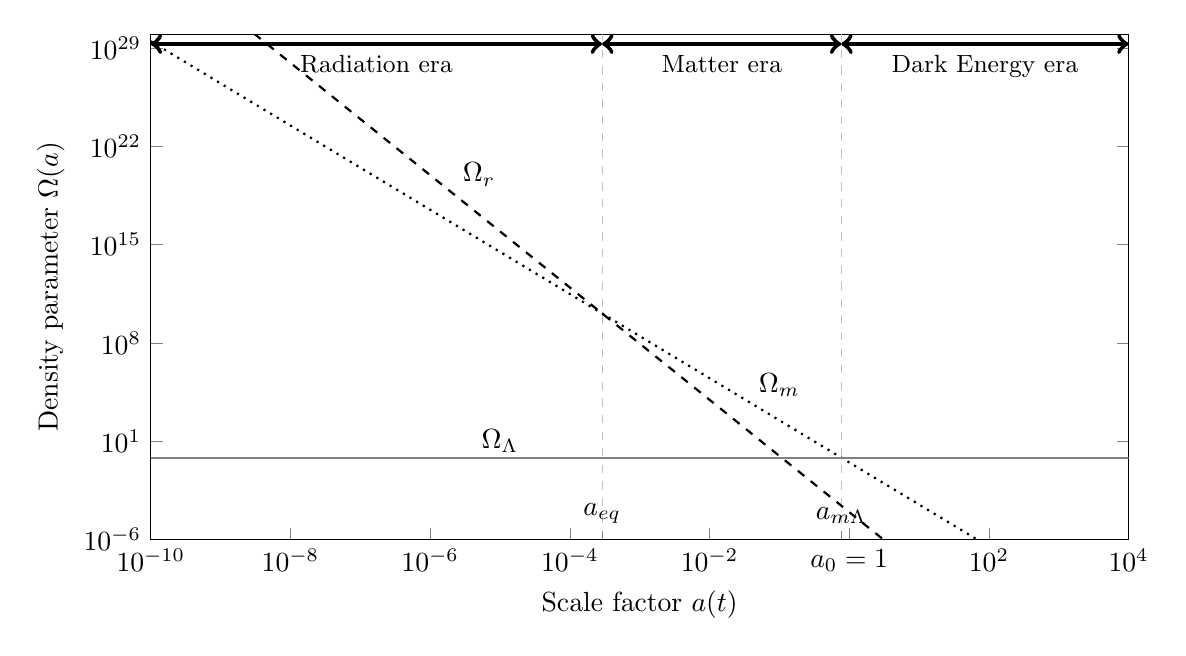
\begin{tikzpicture}
        \begin{axis}[
            width=14cm, height=8cm,
            xlabel={Scale factor $a(t)$}, ylabel={Density parameter $\Omega(a)$},
            xmin=1e-10, xmax=1e4,
            ymin=1e-6, ymax=1e30,
            xmode=log,
            ymode=log,
            extra x ticks={0.77, 2.9e-4},
            extra x tick labels={$a_{m\Lambda}$,$a_\text{eq}$},
            extra x tick style={grid=major, dashed},
            xtick pos = left,
            xtick = {1e-10,1e-8,1e-6,1e-4,1e-2,1,1e2,1e4},
            xticklabels ={$10^{-10}$,$10^{-8}$,$10^{-6}$,$10^{-4}$,$10^{-2}$,$a_0=1$, $10^2$,$10^4$},
            extra x tick style={xticklabel style={yshift=0.5ex, anchor=south}},
        ]
    
            % Radiation density
            \addplot[
                domain=1e-10:1e4,
                samples=200,
                thick,
                dashed
            ] {9*10^(-5)/x^4};
            \node at (axis cs:5e-6,1e20) {$\Omega_r$};
    
            % Matter density
            \addplot[
                domain=1e-10:1e4,
                samples=200,
                thick,
                dotted
            ] {0.31/x^3};
            \node at (axis cs:1e-1,1e5) {$\Omega_m$};
    
            % Vacuum density
            \addplot[
                domain=1e-10:1e4,
                samples=200,
                thick,
                gray
            ] {0.68};
            \node at (axis cs:1e-5,1e1) {$\Omega_\Lambda$};
    
            % Arrows and labels for the eras
            % Radiation-dominated era
            \draw[<->, ultra thick] (axis cs:1e-10,2e29) -- (axis cs:2.9e-4,2e29)
                node[midway, below, font=\small] {Radiation era};
    
            % Matter-dominated era
            \draw[<->,ultra thick] (axis cs:2.9e-4,2e29) -- (axis cs:0.77,2e29)
                node[midway, below, font=\small] {Matter era};
    
            % Dark energy-dominated era
            \draw[<->,ultra thick] (axis cs:0.77,2e29) -- (axis cs:1e4,2e29)
                node[midway, below, font=\small] {Dark Energy era};
    
        \end{axis}
    \end{tikzpicture}
    \caption{Evolution of the densities of matter, radiation and dark energy. In this plot the transitions between the main eras are showed.}
    \label{fig:Universe_history}
\end{figure}

Going further back in time the scale factor continues to decrease ($a_\text{rad}(t)\propto\sqrt{t}$) and we reach a scale at which the universe was so small that quantum mechanics effects must be taken into account and a theory of \emph{quantum gravity} is required. However, no-definitive solution for this problem has been found today.\\ For our purposes we will assume that the history of the universe started when $a=0$, in this way we can convert our redshifts in comoving time. From the Friedmann equation \eqref{eq:Friedmann1} $a(t)$ can be converted in a time by the following integral$$H_0t=\int_{0}^{a}\frac{da'}{\sqrt{\Omega_{r,0}a^{-2}+\Omega_{m,0}a^{-1}+\Omega_{\Lambda,0}a^{2}+\Omega_{k,0}}}\ \Rightarrow\ \begin{cases}
    t_{m\Lambda}\approx10.2\text{Gyrs},\\
    t_0\approx13.8\text{Gyrs},\\
    t_\text{eq}\approx 50\ 000\text{yrs},.
\end{cases}$$
This shows that, compared to the entire life of the universe ($t_0$) the \emph{radiation dominated era} lasted  only for 50 000 years, while the \emph{dark energy dominated era} is the closest to us, that started only a few billion years ago. Then the \emph{matter dominated era} is the longest one of the three. 




